\documentclass[aspectratio=169]{beamer}
\setbeamertemplate{navigation symbols}{}
\usepackage{color, amsmath, comment, subfigure}
\usepackage{url}
\usepackage{ulem}

\usepackage{hyperref}
\hypersetup{
    colorlinks=true,
    linkcolor=blue,
    filecolor=magenta,      
    urlcolor=cyan,
}

%%%%%%%%%%%%%%%%%%%%%%%%%%
\title[]{Pre-read for Thursday, October 24:\\Weather, Empirical}
\author[]{Matthew J. Salganik}
\institute[]{}
\date[]{COS 597E/SOC 555 Limits to prediction\\Fall 2020, Princeton University}

\begin{document}
%%%%%%%%%%%%%%%%%%%%%%%%%%%
\frame{\titlepage}
%%%%%%%%%%%%%%%%%%%%%%%%%%%
\begin{frame}
\frametitle{}

\begin{align*}
  x' &= \sigma(y-x) \\
  y' &= x(\rho-z)-y \\
  z' &= xy-\beta z
\end{align*}
\begin{center}
$\sigma = 10, \rho = 28,  \beta = 8/3$ 
\end{center}
\begin{center}
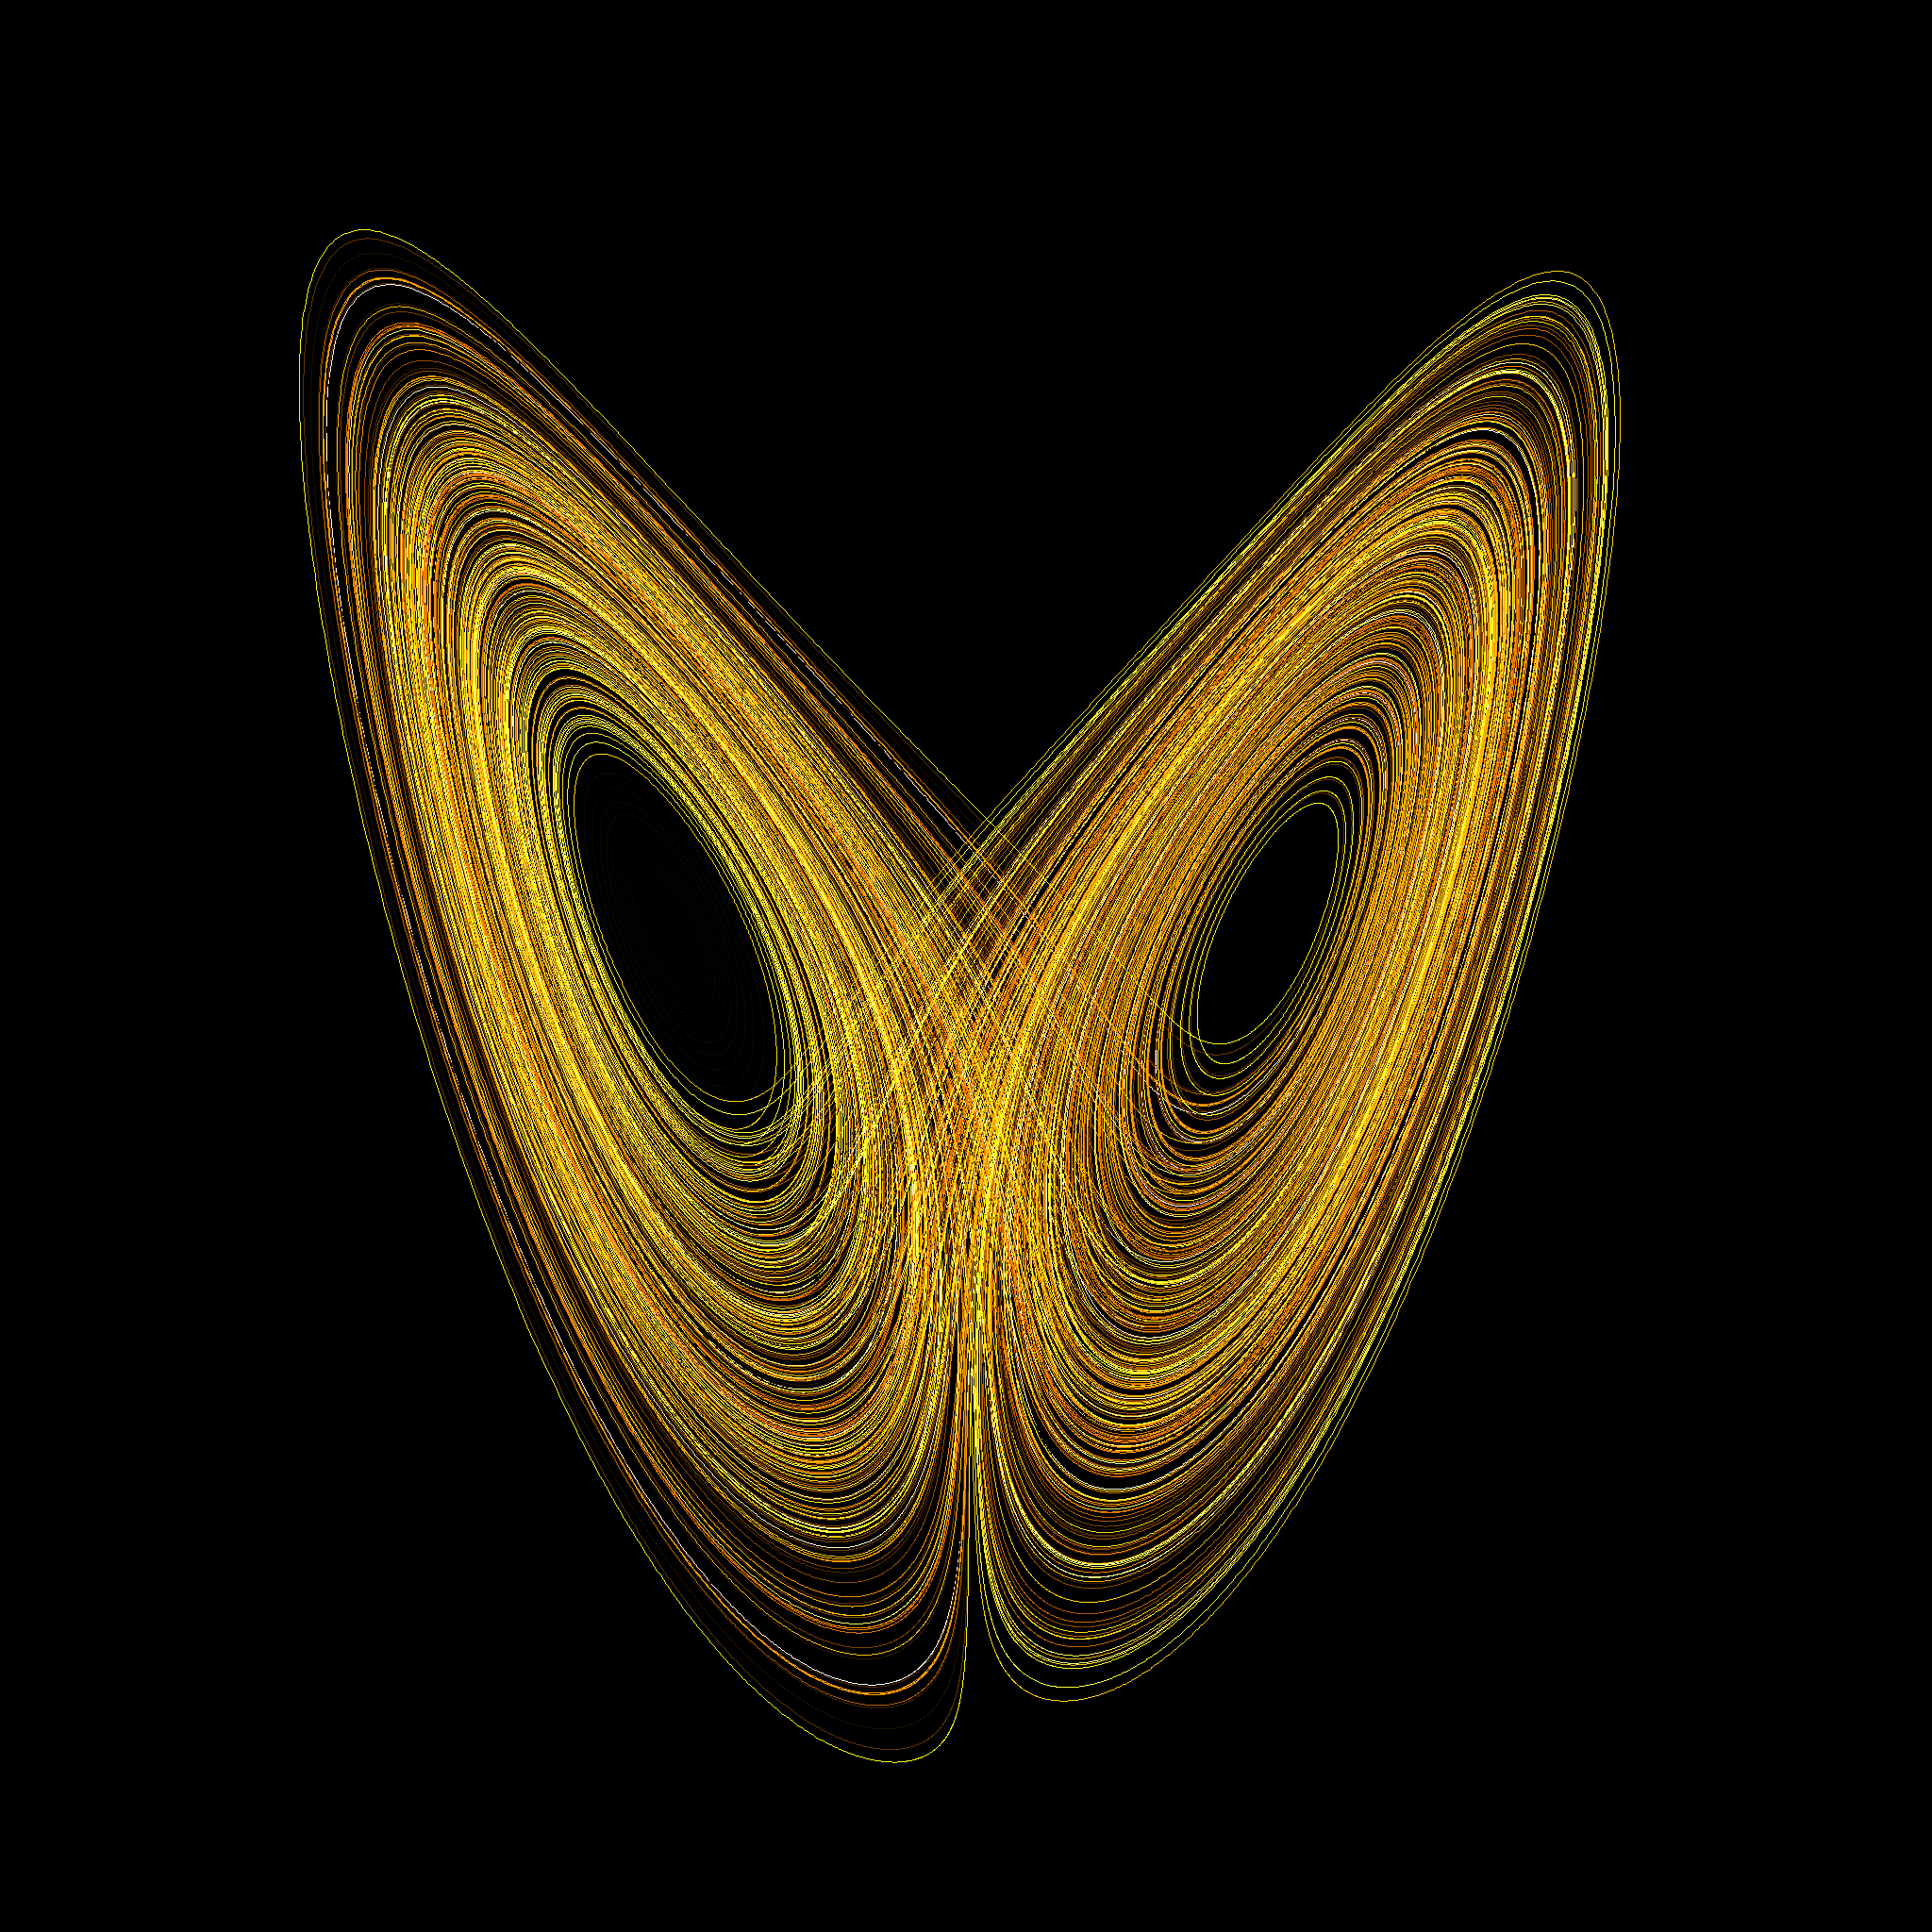
\includegraphics[width = 0.3\textwidth]{figures/Lorenz_system_r28_s10_b2-6666}
\end{center}

\vfill
\tiny{\url{https://commons.wikimedia.org/wiki/File:Lorenz_system_r28_s10_b2-6666.png}}
\end{frame}
%%%%%%%%%%%%%%%%%%%%%%%%%%%%%
\begin{frame}

\begin{center}

\includegraphics[width = 0.9\textwidth]{figures/lorenz_essence_1993_ch3}
\end{center}

\end{frame}
%%%%%%%%%%%%%%%%%%%%%%%%%%%%
\begin{frame}

Reading notes
\begin{itemize}
\item Forecasting the weather vs forecasting the tides, think about how this relates to absolute measures of predictability vs measures relative some baseline.
\pause
\item In the section ``The Unperformable Experiment'' he describes the problems of studying the real atmosphere, and that leads to the reliance of physical models and computer models.  To what extent do we see these same tricks in other areas?
\end{itemize}

\end{frame}
%%%%%%%%%%%%%%%%%%%%%%%%%%%%%
\begin{frame}
\frametitle{}

\begin{center}
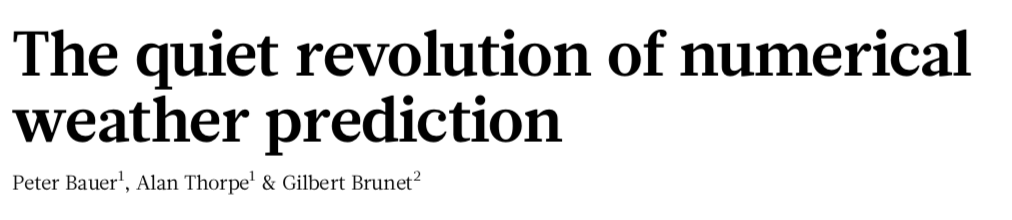
\includegraphics[width = 0.9\textwidth]{figures/bauer_quiet_2015_title}
\end{center}

\end{frame}
%%%%%%%%%%%%%%%%%%%%%%%%%%%%%
\begin{frame}
\frametitle{}

Things I like about numerical weather prediction:
\begin{itemize}
\item Many groups make public predictions every day at multiple time scales (5-day forecast, 10-day forecast), and we can all see how accurate they are
\pause
\item No self-fulfilling or self-defeating processes 
\pause
\item No concerns about causality
\pause
\item Predictions based a real physical model
\pause
\item Business and governments invests in improved performance
\end{itemize}

\end{frame}
%%%%%%%%%%%%%%%%%%%%%%%%%%%%%
\begin{frame}
\frametitle{}

\begin{center}
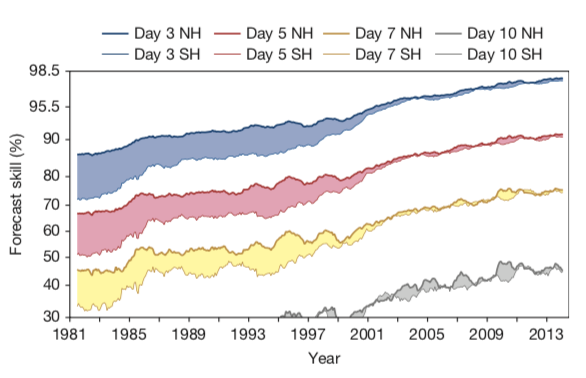
\includegraphics[width = 0.8\textwidth]{figures/bauer_quiet_2015_fig1}
\end{center}

\vfill
This is impressive.

\end{frame}
%%%%%%%%%%%%%%%%%%%%%%%%%%%%%
\begin{frame}
\frametitle{}

\begin{center}
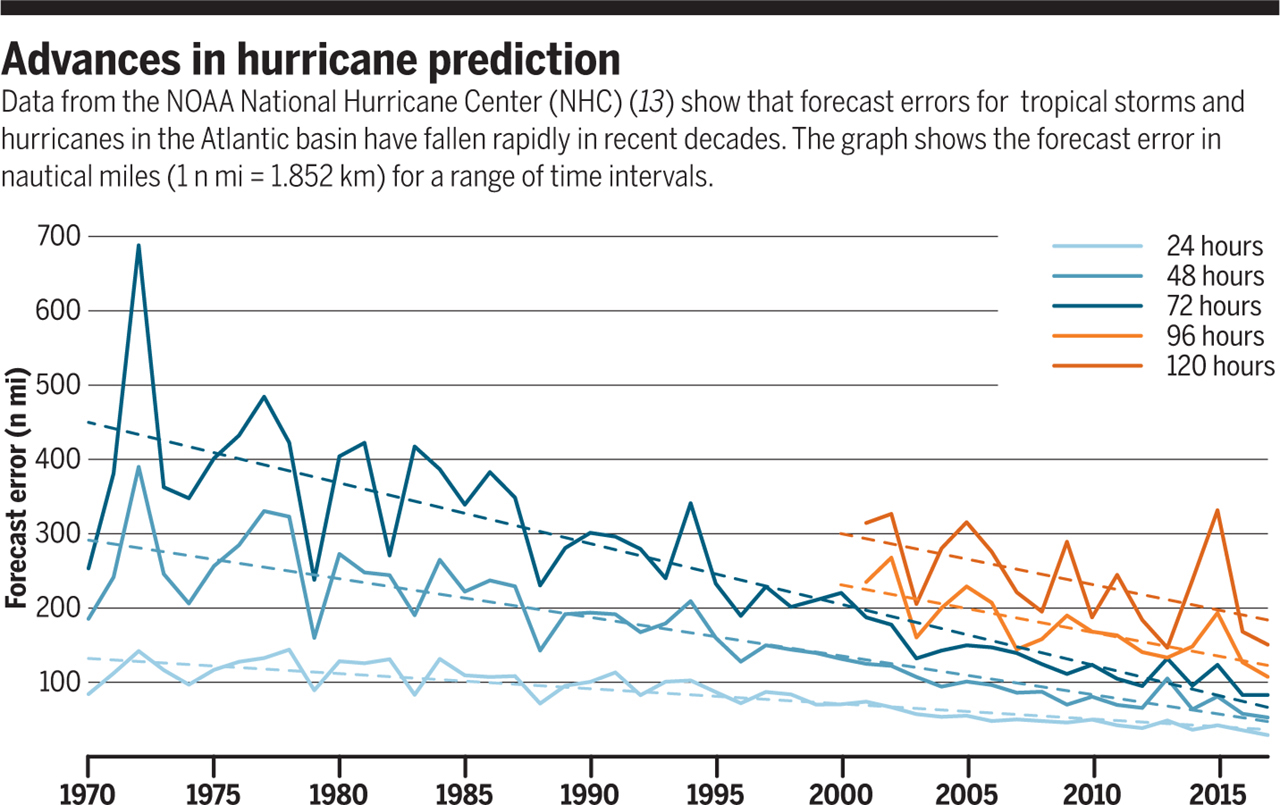
\includegraphics[width = 0.8\textwidth]{figures/alley_advances_2019_fig2}
\end{center}

\vfill
This is impressive. Source: Alley et al 2019

\end{frame}
%%%%%%%%%%%%%%%%%%%%%%%%%%%%%
\begin{frame}
\frametitle{}

\begin{center}
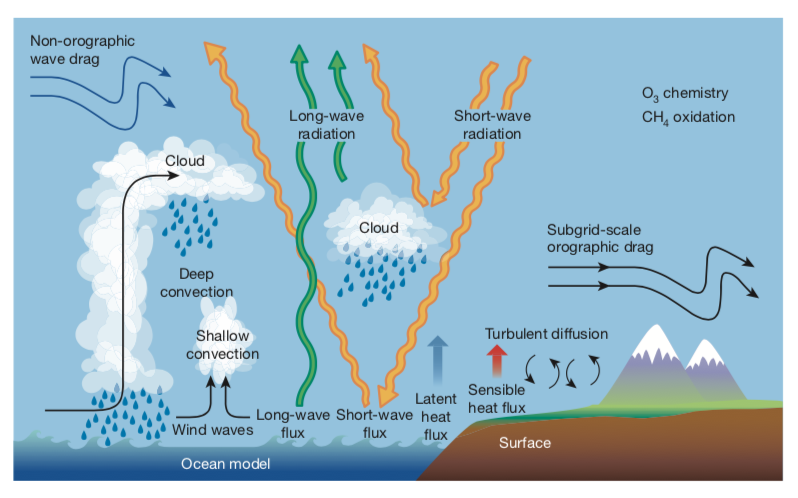
\includegraphics[width = 0.9\textwidth]{figures/bauer_quiet_2015_fig2}
\end{center}

\vfill
Note the many interacting systems involved.

\end{frame}
%%%%%%%%%%%%%%%%%%%%%%%%%%%%%
\begin{frame}
\frametitle{}

\begin{center}
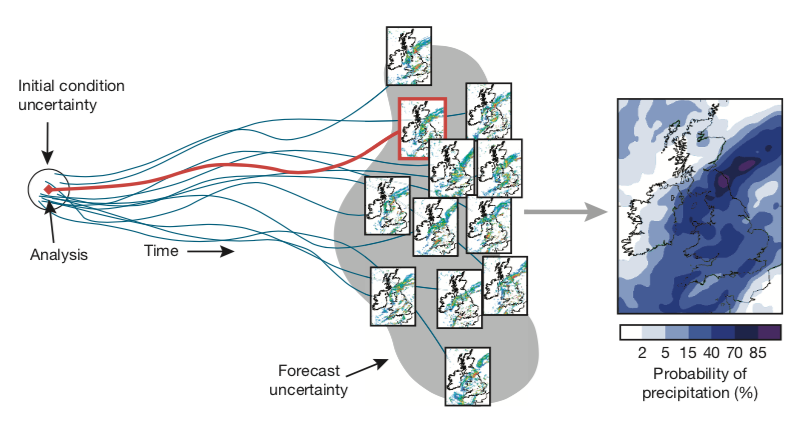
\includegraphics[width = 0.9\textwidth]{figures/bauer_quiet_2015_fig3}
\end{center}

\vfill
Sensitive dependences does not make them quit.

\end{frame}
%%%%%%%%%%%%%%%%%%%%%%%%%%%%%
\begin{frame}

\begin{center}
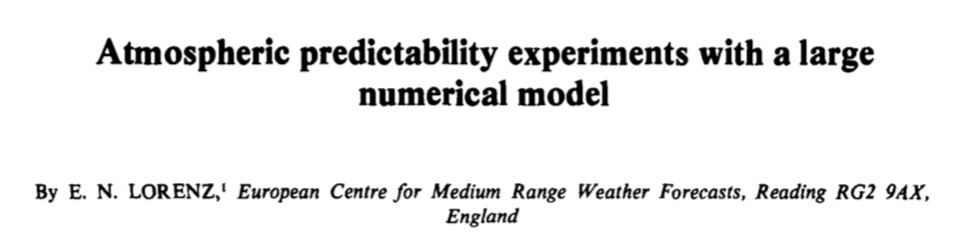
\includegraphics[width = 0.9\textwidth]{figures/lorenz_atmospheric_1982_title}
\end{center}

\vfill
Upper and lower bound on predictability with no extra computing!  

\end{frame}
%%%%%%%%%%%%%%%%%%%%%%%%%%%%%
\begin{frame}
\frametitle{}

We want to understand the upper bound and lower bound for accuracy using the model from the European Center for Medium Range Weather Forecasts (ECMWF) 
\begin{itemize}
\item How accurate are predictions?  This gives lower bound on accuracy.
\pause
\item How much do two similar initial conditions diverge?  This gives an upper bound on accuracy.
\end{itemize}


We'd like to do this without running the model many times because running the model is expensive.

\end{frame}
%%%%%%%%%%%%%%%%%%%%%%%%%%%%%
\begin{frame}
\frametitle{}

Model produces ``prognoses'':
\begin{itemize}
\item 1 Dec: 0 day, 1 day, 2 days $\ldots$, 10 days
\item 2 Dec: 0 day, 1 day, 2 days $\ldots$, 10 days
\item 3 Dec: 0 day, 1 day, 2 days $\ldots$, 10 days
\item $\vdots$
\item 10 March: 0 day, 1 day, 2 days $\ldots$, 10 days
\end{itemize}
\end{frame}
%%%%%%%%%%%%%%%%%%%%%%%%%%%%%
\begin{frame}
\frametitle{}

\begin{itemize}
\item 1 Dec: 0 day (1 Dec), 1 day (2 Dec), 2 days (3 Dec) $\ldots$, 10 days (11 Dec)
\pause
\item 2 Dec: 0 day (2 Dec), 1 day (3 Dec), 2 days (4 Dec) $\ldots$, 10 days (12 Dec)
\pause
\item 3 Dec: 0 day (3 Dec), 1 day (4 Dec), 2 days (5 Dec) $\ldots$, 10 days (13 Dec)
\pause
\item 4 Dec: 0 day (4 Dec), 1 day (5 Dec), 2 days (6 Dec) $\ldots$, 10 days (14 Dec)
\item $\vdots$
\end{itemize}

\end{frame}
%%%%%%%%%%%%%%%%%%%%%%%%%%%%%
\begin{frame}
\frametitle{}

How accurate are 1 day forecasts? This is equivalent to asking:  What is $E_{01}$?
\begin{itemize}
\item 1 Dec: 0 day (1 Dec), \textcolor{blue}{1 day (2 Dec)}, 2 days (3 Dec) $\ldots$, 10 days (11 Dec)
\item 2 Dec: \textcolor{blue}{0 day (2 Dec)}, 1 day (3 Dec), 2 days (4 Dec) $\ldots$, 10 days (12 Dec)
\item 3 Dec: 0 day (3 Dec), 1 day (4 Dec), 2 days (5 Dec) $\ldots$, 10 days (13 Dec)
\item 4 Dec: 0 day (4 Dec), 1 day (5 Dec), 2 days (6 Dec) $\ldots$, 10 days (14 Dec)
\item $\vdots$
\end{itemize}

\end{frame}
%%%%%%%%%%%%%%%%%%%%%%%%%%%%%
\begin{frame}
\frametitle{}

How accurate are 1 day forecasts? This is equivalent to asking:  What is $E_{01}$?
\begin{itemize}
\item 1 Dec: 0 day (1 Dec), 1 day (2 Dec), 2 days (3 Dec) $\ldots$, 10 days (11 Dec)
\item 2 Dec: 0 day (2 Dec), \textcolor{blue}{1 day (3 Dec)}, 2 days (4 Dec) $\ldots$, 10 days (12 Dec)
\item 3 Dec: \textcolor{blue}{0 day (3 Dec)}, 1 day (4 Dec), 2 days (5 Dec) $\ldots$, 10 days (13 Dec)
\item 4 Dec: 0 day (4 Dec), 1 day (5 Dec), 2 days (6 Dec) $\ldots$, 10 days (14 Dec)
\item $\vdots$
\end{itemize}

\end{frame}
%%%%%%%%%%%%%%%%%%%%%%%%%%%%%
\begin{frame}
\frametitle{}

How accurate are 2 day forecasts? This is equivalent to asking:  What is $E_{02}$?
\begin{itemize}
\item 1 Dec: 0 day (1 Dec), 1 day (2 Dec), \textcolor{blue}{2 days (3 Dec)} $\ldots$, 10 days (11 Dec)
\item 2 Dec: 0 day (2 Dec), 1 day (3 Dec), 2 days (4 Dec) $\ldots$, 10 days (12 Dec)
\item 3 Dec: \textcolor{blue}{0 day (3 Dec)}, 1 day (4 Dec), 2 days (5 Dec) $\ldots$, 10 days (13 Dec)
\item 4 Dec: 0 day (4 Dec), 1 day (5 Dec), 2 days (6 Dec) $\ldots$, 10 days (14 Dec)
\item $\vdots$
\end{itemize}

\end{frame}
%%%%%%%%%%%%%%%%%%%%%%%%%%%%%
\begin{frame}
\frametitle{}

How accurate are 2 day forecasts? This is equivalent to asking:  What is $E_{02}$?
\begin{itemize}
\item 1 Dec: 0 day (1 Dec), 1 day (2 Dec), 2 days (3 Dec) $\ldots$, 10 days (11 Dec)
\item 2 Dec: 0 day (2 Dec), 1 day (3 Dec), \textcolor{blue}{2 days (4 Dec)} $\ldots$, 10 days (12 Dec)
\item 3 Dec: 0 day (3 Dec), 1 day (4 Dec), 2 days (5 Dec) $\ldots$, 10 days (13 Dec)
\item 4 Dec: \textcolor{blue}{0 day (4 Dec)}, 1 day (5 Dec), 2 days (6 Dec) $\ldots$, 10 days (14 Dec)
\item $\vdots$
\end{itemize}

\end{frame}
%%%%%%%%%%%%%%%%%%%%%%%%%%%%%
\begin{frame}

\begin{center}
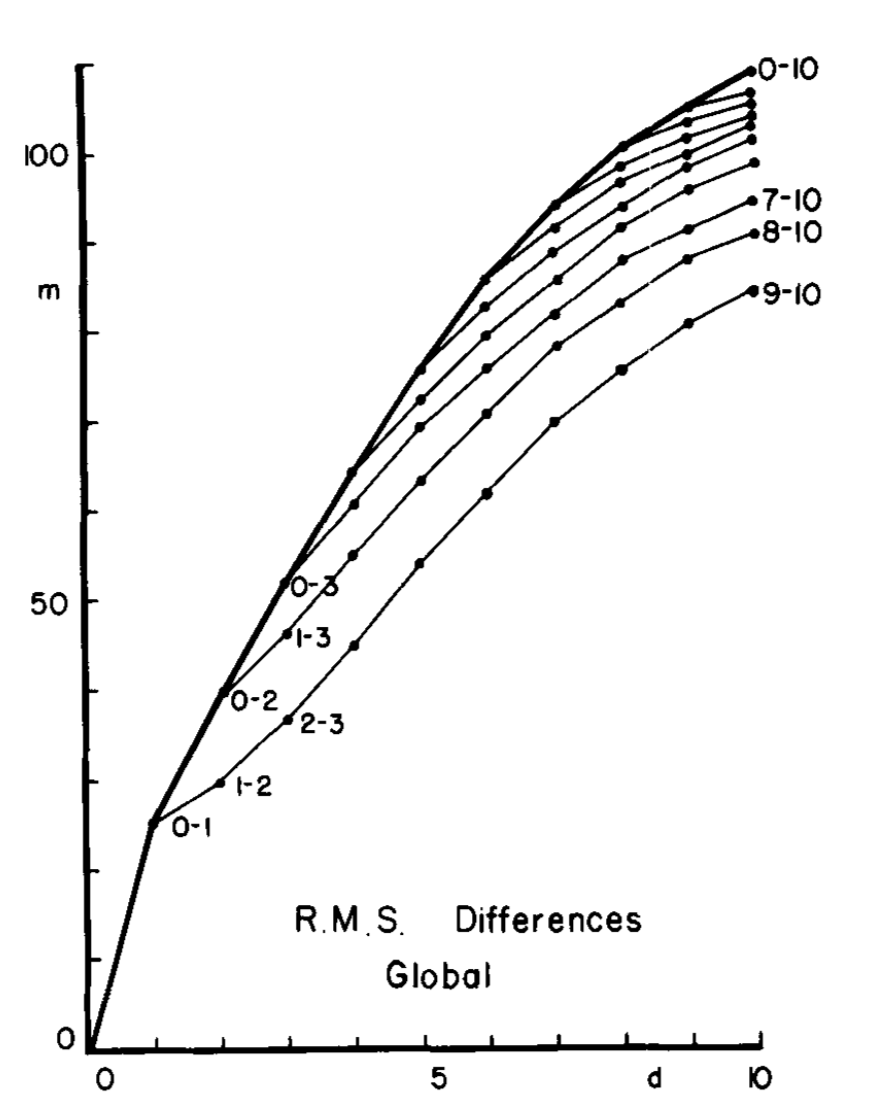
\includegraphics[height = 0.8\textheight]{figures/lorenz_atmospheric_1982_fig1}
\end{center}

\vfill
$E_{01}, E_{02}, \ldots E_{010}$ is the heavy curve at the top

\end{frame}
%%%%%%%%%%%%%%%%%%%%%%%%%%%%%
\begin{frame}

What about two trajectories that start close together?  How fast do they diverge?

\end{frame}
%%%%%%%%%%%%%%%%%%%%%%%%%%%%%
\begin{frame}
\frametitle{}

\begin{itemize}
\item 1 Dec: 0 day (1 Dec), \textcolor{red}{1 day (2 Dec)}, \textcolor{blue}{2 days (3 Dec)} $\ldots$
\item 2 Dec: \textcolor{red}{0 day (2 Dec)}, \textcolor{blue}{1 day (3 Dec)}, 2 days (4 Dec) $\ldots$
\item 3 Dec: 0 day (3 Dec), 1 day (4 Dec), 2 days (5 Dec) $\ldots$ 
\item 4 Dec: 0 day (4 Dec), 1 day (5 Dec), 2 days (6 Dec) $\ldots$
\item $\vdots$
\end{itemize}

\pause

\vfill
Distance between \textcolor{red}{0 day (2 Dec)} and \textcolor{red}{1 day (2 Dec)}: $\epsilon$\\
\pause
Distance between \textcolor{blue}{1 day (3 Dec)} and  \textcolor{blue}{2 days (3 Dec)}: $c \cdot \epsilon$ for $(c > 1)$

\end{frame}
%%%%%%%%%%%%%%%%%%%%%%%%%%%%%
\begin{frame}
\frametitle{}

\begin{itemize}
\item 1 Dec: 0 day (1 Dec), 1 day (2 Dec), 2 days (3 Dec) $\ldots$
\item 2 Dec: 0 day (2 Dec), \textcolor{red}{1 day (3 Dec)}, \textcolor{blue}{2 days (4 Dec)} $\ldots$
\item 3 Dec: \textcolor{red}{0 day (3 Dec)}, \textcolor{blue}{1 day (4 Dec)}, 2 days (5 Dec) $\ldots$
\item 4 Dec: 0 day (4 Dec), 1 day (5 Dec), 2 days (6 Dec) $\ldots$
\item $\vdots$
\end{itemize}

\pause
\vfill
\onslide<2->{Distance between \textcolor{red}{0 day (3 Dec)} and \textcolor{red}{1 day (3 Dec)}: $\epsilon$} \onslide<4->{$(E_{01})$} \\
\onslide<3->{Distance between \textcolor{blue}{1 day (4 Dec)} and \textcolor{blue}{2 days (4 Dec)}: $c \cdot \epsilon$ for $(c > 1)$} \onslide<5->{$(E_{12})$}

\end{frame}
%%%%%%%%%%%%%%%%%%%%%%%%%%%%%
\begin{frame}
\frametitle{}

\begin{itemize}
\item 1 Dec: 0 day (1 Dec), 1 day (2 Dec), 2 days (3 Dec), 3 days (4 Dec) $\ldots$
\item 2 Dec: 0 day (2 Dec), \textcolor{red}{1 day (3 Dec)}, 2 days (4 Dec), \textcolor{blue}{3 days (5 Dec)} $\ldots$
\item 3 Dec: \textcolor{red}{0 day (3 Dec)}, 1 day (4 Dec), \textcolor{blue}{2 days (5 Dec)} 3 days (6 Dec) $\ldots$
\item 4 Dec: 0 day (4 Dec), 1 day (5 Dec), 2 days (6 Dec), 3 days (7 Dec) $\ldots$
\item $\vdots$
\end{itemize}

\pause
\vfill
\onslide<2->{Distance between \textcolor{red}{0 day (3 Dec)} and \textcolor{red}{1 day (3 Dec)}: $\epsilon$} \onslide<4->{$(E_{01})$} \\
\onslide<3->{Distance between \textcolor{blue}{2 day (5 Dec)} and \textcolor{blue}{3 days (5 Dec)}: $c \cdot \epsilon$ for $(c > 1)$} \onslide<5->{$(E_{23})$}

\end{frame}
%%%%%%%%%%%%%%%%%%%%%%%%%%%%%
\begin{frame}

\begin{center}
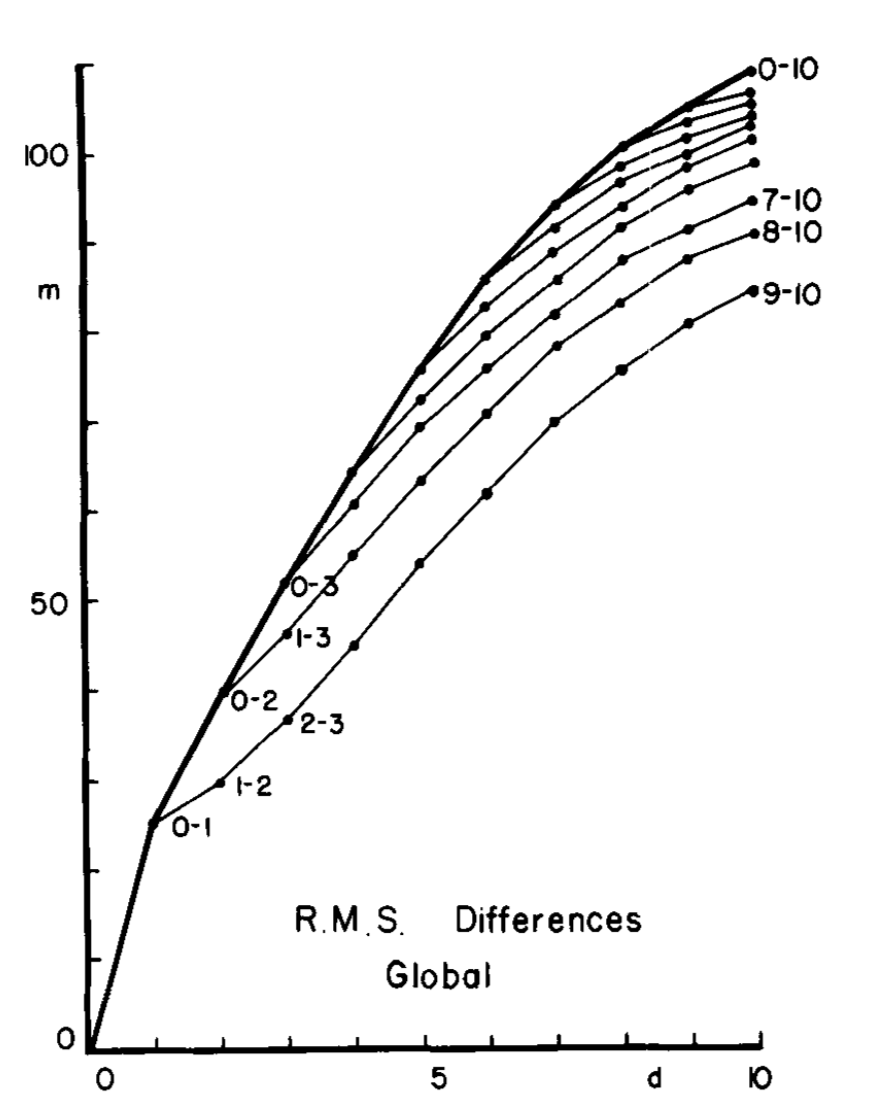
\includegraphics[height = 0.8\textheight]{figures/lorenz_atmospheric_1982_fig1}
\end{center}

\vfill
$E_{12}, E_{23}, \ldots E_{910}$ is the light curve at the bottom

\end{frame}
%%%%%%%%%%%%%%%%%%%%%%%%%%%%%
\begin{frame}

\onslide<1>{What about two trajectories that start close together?  How fast do they diverge?}\\
\onslide<2->{\sout{What about two trajectories that start close together?  How fast do they diverge?}}
\onslide<2->{What about two trajectories that start a bit further apart?  How fast do they diverge?}

\end{frame}
%%%%%%%%%%%%%%%%%%%%%%%%%%%%%
\begin{frame}
\frametitle{}

\small{
\begin{itemize}
\item 1 Dec: 0 day (1 Dec), 1 day (2 Dec), \textcolor{red}{2 days (3 Dec)}, \textcolor{blue}{3 days (4 Dec)}, 4 days (5 Dec) $\ldots$
\item 2 Dec: 0 day (2 Dec), 1 day (3 Dec), 2 days (4 Dec), 3 days (5 Dec), 4 days (6 Dec) $\ldots$
\item 3 Dec: \textcolor{red}{0 day (3 Dec)}, \textcolor{blue}{1 day (4 Dec)}, 2 days (5 Dec), 3 days (6 Dec), 4 days (7 Dec) $\ldots$
\item 4 Dec: 0 day (4 Dec), 1 day (5 Dec), 2 days (6 Dec), 3 days (7 Dec), 4 days (8 Dec) $\ldots$
\item $\vdots$
\end{itemize}
}

\vfill

\onslide<2->{Distance between \textcolor{red}{0 day (3 Dec)} and \textcolor{red}{2 day (3 Dec)}: $\epsilon$} \onslide<4->{$(E_{02})$} \\
\onslide<3->{Distance between \textcolor{blue}{1 day (4 Dec)} and \textcolor{blue}{3 days (4 Dec)}: $c \cdot \epsilon$ for $(c > 1)$} \onslide<5->{$(E_{13})$}\\

\end{frame}
%%%%%%%%%%%%%%%%%%%%%%%%%%%%%
\begin{frame}
\frametitle{}

\small{
\begin{itemize}
\item 1 Dec: 0 day (1 Dec), 1 day (2 Dec), \textcolor{red}{2 days (3 Dec)}, 3 days (4 Dec), \textcolor{blue}{4 days (5 Dec)}  $\ldots$
\item 2 Dec: 0 day (2 Dec), 1 day (3 Dec), 2 days (4 Dec), 3 days (5 Dec), 4 days (6 Dec)  $\ldots$
\item 3 Dec: \textcolor{red}{0 day (3 Dec)}, 1 day (4 Dec), \textcolor{blue}{2 days (5 Dec)}, 3 days (6 Dec), 4 days (7 Dec) $\ldots$
\item 4 Dec: 0 day (4 Dec), 1 day (5 Dec), 2 days (6 Dec),  3 days (7 Dec), 4 days (8 Dec) $\ldots$
\item $\vdots$
\end{itemize}
}

\vfill
\onslide<2->{Distance between \textcolor{red}{0 day (3 Dec)} and \textcolor{red}{2 day (3 Dec)}: $\epsilon$} \onslide<4->{$(E_{02})$} \\
\onslide<3->{Distance between \textcolor{blue}{2 day (5 Dec)} and \textcolor{blue}{4 days (5 Dec)}: $c \cdot \epsilon$ for $(c > 1)$} \onslide<5->{$(E_{24})$}

\end{frame}
%%%%%%%%%%%%%%%%%%%%%%%%%%%%%
\begin{frame}

\begin{center}
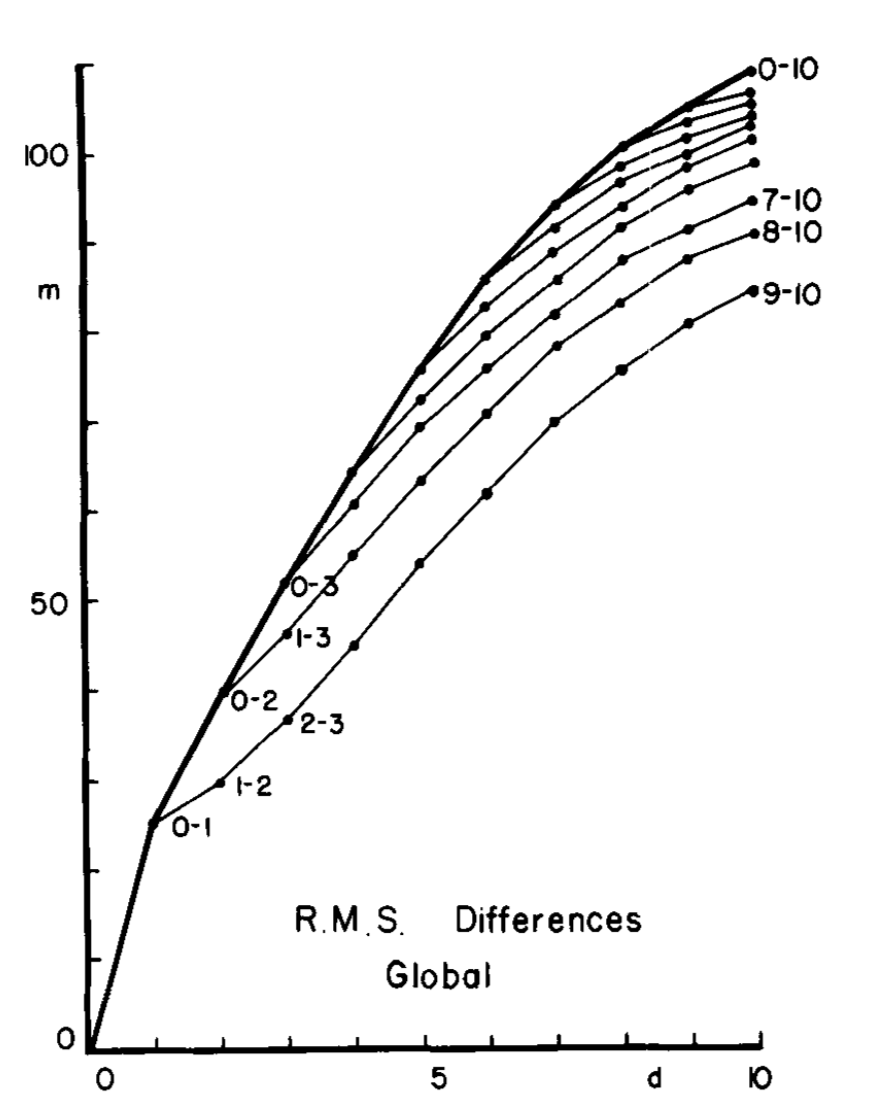
\includegraphics[height = 0.8\textheight]{figures/lorenz_atmospheric_1982_fig1}
\end{center}

\vfill
$E_{12}, E_{23}, \ldots E_{910}$ is the light curve second from the bottom

\end{frame}
%%%%%%%%%%%%%%%%%%%%%%%%%%%%%
\begin{frame}

What can we learn from this figure?

\begin{center}
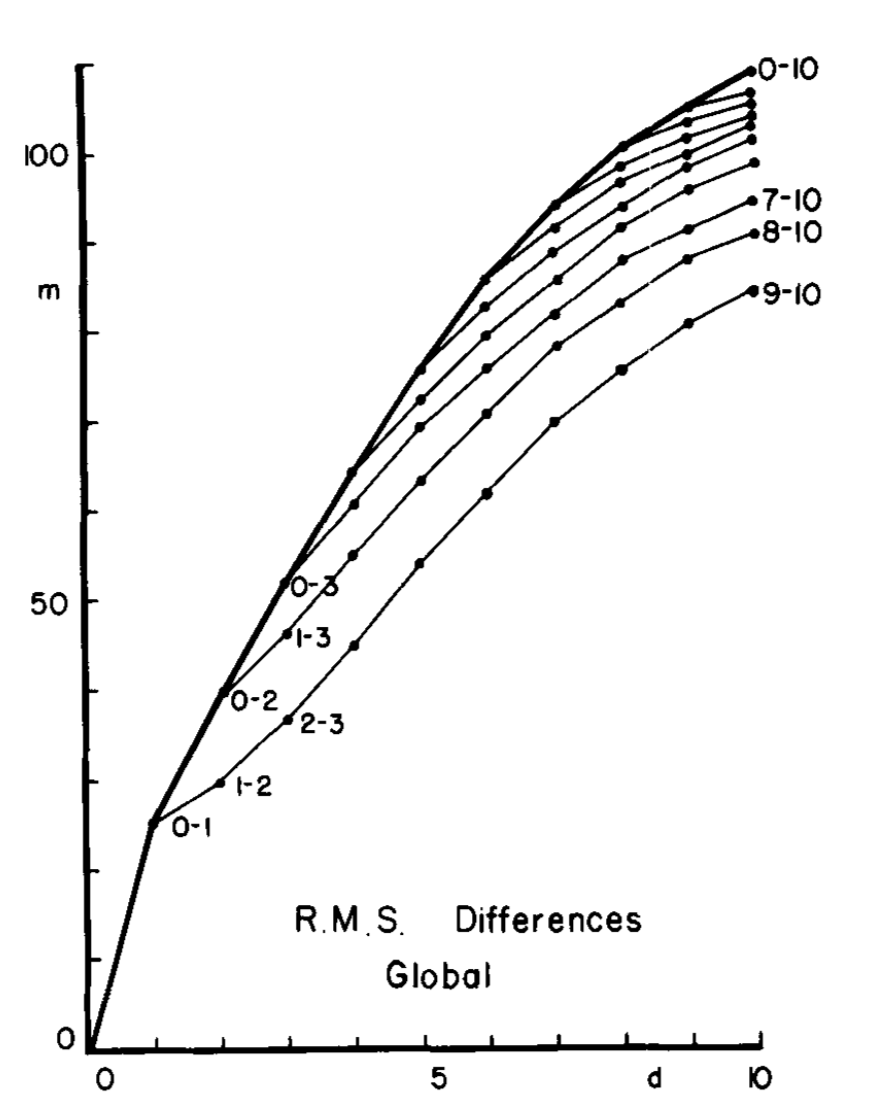
\includegraphics[height = 0.8\textheight]{figures/lorenz_atmospheric_1982_fig1}
\end{center}

\end{frame}
%%%%%%%%%%%%%%%%%%%%%%%%%%%%%
\frame{\titlepage}


\end{document}
